\documentclass[a4paper]{article}

%% Language and font encodings
\usepackage{polski}
\usepackage[polish]{babel}
\usepackage[utf8x]{inputenc}
\usepackage[T1]{fontenc}
\usepackage{pdfpages}
\usepackage{indentfirst}
\usepackage{listings}
\usepackage{isotope}

\usepackage{csvsimple}
\setlength{\tabcolsep}{2pt}

% Adjust penalties
\brokenpenalty=1000
\clubpenalty=1000
\widowpenalty=1000

% Don't break in math expressions
\relpenalty=10000
\binoppenalty=10000

%% Sets page size and margins
\usepackage[a4paper]{geometry}

%% Useful packages
\usepackage{amsmath}
\usepackage{graphicx}
\usepackage[colorlinks=true, allcolors=blue]{hyperref}
\usepackage{booktabs}
\usepackage{cancel}
\usepackage{tikz}

\usepackage{float}

\renewcommand\thesection{\arabic{section}.}
\renewcommand\thesubsection{\arabic{section}.\arabic{subsection}.}
\renewcommand\thesubsubsection{\arabic{section}.\arabic{subsection}.\arabic{subsubsection}.}

% The following commands are not supported in PSTricks at present
% We define them conditionally, so when they are implemented,
% this pgf file will use them.
\ifx\du\undefined
  \newlength{\du}
\fi
\setlength{\du}{15\unitlength}

\newcommand{\Vsp}[1]{\vtop to #1 {}}
\newcommand{\Hsp}[1]{\hbox to #1 {}}
\newcommand{\Small}{\scriptsize}

\title{Sprawozdanie nr 7}
\date{}


\begin{document}

\begin{center}
\begin{tabular}{|p{5.5cm}|l|l|c|}
    \hline
	% Row 1.1  
	    Wydział \Vsp{4mm} &
	    \multicolumn{1}{|l}{Dzień} &
	    poniedziałek $17^{15} - 19^{30}$ &
	    Nr zespołu \\
	% Row 1.2
	    \mbox{\small{Matematyki i Nauk Informatycznych}} &
	    \multicolumn{1}{|l}{Data}  &
	    &
	    \multicolumn{1}{c|}{\Large{18}} \\
    
    \hline
	% Row 2.1 
	    Nazwisko i Imię: &
	    \Small Ocena z przygotowania &
	    \Small Ocena ze sprawozdania &
	    \Small Ocena Końcowa \\
	% Rows 2.2-2.4
	    1. Jasiński Bartosz & & &\\
	    2. Sadłocha Adrian & & & \\
	    3. Wódkiewicz Andrzej & & & \\

    \hline
    % Row 3.1
	    \multicolumn{2}{|l|}{Prowadzący \Vsp{4mm}} &
	    \multicolumn{2}{|l|}{Podpis prowadzącego} \\  
    % Row 3.2
    	\multicolumn{2}{|l|}{dr hab. Katarzyna Grebieszkow} &
    	\multicolumn{2}{|l|}{} \\    	
    \hline
\end{tabular}
\label{pieczatka}
\end{center}

{\let\newpage\relax\maketitle}
\setcounter{secnumdepth}{2}


\section{Opis ćwiczenia}

Celem ćwiczenia jest weryfikacja hipotezy de Broglie'a.
Hipoteza ta głosi, że wszelka materia ma dwojaką naturę: cząsteczkową oraz falową.

\subsection{Wstęp teoretyczny}

Według przedstawionej hipotezy, każdej cząstce można przypisać falę o pewnej długości.
Jeśli przez $h$ oznaczmy stałą Plancka, zaś przez $p$ pęd cząstki, to długość fali de Broglie'a (ozn. $\lambda$) jest definiowana jako:

$$\lambda = \frac h p$$

% TODO: lepsze wyjaśnienie hipotezy de Broglie'a
% TODO: wyprowadzenie potrzebnych wzorów/wzoru
% TODO: wyjaśnienie skąd jest „dwójka” we wzorze
% TODO: doświadczenie Thomsona

\subsection{Układ pomiarowy}

Do weryfikacji hipotezy de Broglie'a użyta została lampa oscyloskopowa oraz cienka folia grafitowa.
W celu przyspieszania elektronów przykładane było regulowane napięcie.
Do odczytu napięcia służył cyfrowy wyświetlacz o rozdzielczości wynoszącej $0.01$ kV.

Odległość pomiędzy folią grafitową a ekranem wynosiła -- zgodnie z instrukcją -- $127$ $(3)$ mm.

% TODO: uzupełnić

\section{Pomiary i wstępne obliczenia}

Dokonaliśmy dwóch serii pomiarów, kolejno $A$ oraz $B$.
W obu seriach napięcie (ozn. $U$) ustalane było między ok. $3.50$ kV a ok. $11.10$ kV, z różnicą ok. $0.40$ kV pomiędzy pomiarami.
Podczas serii $A$ napięcie rosło wraz z każdym pomiarem, podczas serii $B$ -- malało.

Ponieważ stan podczas odczytu napięcia nie był stabilny (największy zauważony przez nas skok wartości wyniósł $0.09$ kV), za niepewność całkowitą pomiaru $U$ przyjęliśmy:

$$u(U) = \frac{0.09 \, \text{kV}}{\sqrt 3}$$

W dalszej części będziemy sprawdzać zależność liniową pomiędzy średnicą pierścieni a odwrotnością pierwiastka napięcia.
Wprowadźmy oznaczenie $X = \frac{1}{\sqrt U}$ oraz wyliczmy -- korzystając z prawa propagacji niepewności -- niepewność całkowitą:

$$u(X) = \sqrt{\left(\frac{\partial X}{\partial U}\right)^2 \cdot u^2(U)} = \left| -\frac{1}{2 \sqrt{U^3}} \cdot u(U)\right| = \frac{0.09 \, \text{kV}}{2 \sqrt{3} \sqrt{U^3}}$$

Dla ustalonego napięcia interesowała nas średnica najbardziej wewnętrznego pierścienia, ozn.~$D$.
W celu wyznaczenia tej wartości, mierzona była średnica wewnętrzna oraz zewnętrzna pierścienia, oznaczane kolejno $D_w$ oraz~$D_z$.
Za średnicę właściwą przyjęliśmy średnią arytmetyczną z powyższych wartości, tj.~$D = \frac {D_w + D_z}{2}$.

Użyty przyrząd pomiarowy miał podziałkę wynoszącą $\Delta D_w = 1$ mm.
Ze względu na rozmycie pierścieni, za niepewność eksperymentatora przyjęliśmy dwukrotność podziałki: $\Delta D_{w_E} = 2 \cdot \Delta D_w = 2$~mm.
Zatem niepewność całkowita pomiaru średnicy wewnętrznej (a także zewnętrznej, którą oznaczymy przez $u(D_z)$) wynosi:

$$u(D_w) = \sqrt{\frac{\Delta D_w^2}{3} + \frac{\Delta D_{w_E}^2}{3}} = \sqrt \frac{5}{3} \Delta D_w = \sqrt \frac{5}{3} \, \text{mm}$$

Nas jednak interesuje niepewność średnicy właściwej.
Skoro $D = \frac {D_w + D_z}{2}$, to -- ponownie korzystając z prawa propagacji niepewności -- niepewność całkowita pomiaru średnicy wynosi:

$$u(D) = \sqrt{\left(\frac{\partial D}{\partial D_w}\right)^2 \cdot u^2(D_w) + \left(\frac{\partial D}{\partial D_w}\right)^2 \cdot u^2(D_z)} = \sqrt{\frac{1}{4} u^2(D_w) + \frac{1}{4} u^2(D_z)} = \frac{u(D_w)}{\sqrt{2}}$$

Po podstawieniu wyliczonej wcześniej niepewności otrzymujemy:

$$u(D) = \sqrt \frac{5}{6} \, \text{mm} \approx 0.912870929175 \, \text{mm} \approx 1 \, \text{mm}$$

Wyniki pomiarów oraz wstępnych obliczeń zostały przedstawione w Tablicy \ref{seria_A} oraz w Tablicy \ref{seria_B}.
Dla $X$ prezentujemy odpowiednio zaokrąglone wartości z dokładnością do pięciu miejsc po przecinku, zaś obliczenia przeprowadzamy z pełną dostępną precyzją.

\begin{table}
\centering

\begin{tabular}{lrrrrr}
\toprule
L.p. &  $D_w$ (mm) &  $D_z$ (mm) &  $U$ (kV) &  $D$ (mm) &  $X$ ($\frac{1}{\sqrt{kV}}$) \\
\midrule
1  &          22 &          28 &      3.51 &      25.0 &                     0.53376 \\
2  &          20 &          28 &      3.90 &      24.0 &                     0.50637 \\
3  &          17 &          27 &      4.30 &      22.0 &                     0.48224 \\
4  &          19 &          25 &      4.71 &      22.0 &                     0.46078 \\
5  &          17 &          20 &      5.09 &      18.5 &                     0.44324 \\
6  &          17 &          23 &      5.50 &      20.0 &                     0.42640 \\
7  &          16 &          22 &      5.94 &      19.0 &                     0.41031 \\
8  &          16 &          21 &      6.30 &      18.5 &                     0.39841 \\
9  &          14 &          20 &      6.70 &      17.0 &                     0.38633 \\
10 &          13 &          19 &      7.11 &      16.0 &                     0.37503 \\
11 &          14 &          18 &      7.50 &      16.0 &                     0.36515 \\
12 &          13 &          18 &      7.92 &      15.5 &                     0.35534 \\
13 &          14 &          18 &      8.29 &      16.0 &                     0.34731 \\
14 &          13 &          18 &      8.69 &      15.5 &                     0.33923 \\
15 &          14 &          18 &      9.10 &      16.0 &                     0.33150 \\
16 &          13 &          18 &      9.50 &      15.5 &                     0.32444 \\
17 &          13 &          17 &      9.90 &      15.0 &                     0.31782 \\
18 &          12 &          17 &     10.30 &      14.5 &                     0.31159 \\
19 &          12 &          17 &     10.69 &      14.5 &                     0.30585 \\
20 &          12 &          17 &     11.10 &      14.5 &                     0.30015 \\
\bottomrule
\end{tabular}

\caption{Wyniki pomiarów serii $A$ wraz z wyliczonymi wartościami $D$ oraz $X$.}
\label{seria_A}
\end{table}

\begin{table}
\centering

\begin{tabular}{lrrrrr}
\toprule
L.p. &  $D_w$ (mm) &  $D_z$ (mm) &  $U$ (kV) &  $D$ (mm) &  $X$ ($\frac{1}{\sqrt{kV}}$) \\
\midrule
1  &          14 &          16 &     11.10 &      15.0 &                     0.30015 \\
2  &          14 &          17 &     10.69 &      15.5 &                     0.30585 \\
3  &          14 &          16 &     10.30 &      15.0 &                     0.31159 \\
4  &          14 &          18 &      9.89 &      16.0 &                     0.31798 \\
5  &          14 &          18 &      9.50 &      16.0 &                     0.32444 \\
6  &          15 &          18 &      9.10 &      16.5 &                     0.33150 \\
7  &          14 &          18 &      8.70 &      16.0 &                     0.33903 \\
8  &          15 &          18 &      8.30 &      16.5 &                     0.34711 \\
9  &          15 &          19 &      7.89 &      17.0 &                     0.35601 \\
10 &          15 &          19 &      7.50 &      17.0 &                     0.36515 \\
11 &          16 &          19 &      7.10 &      17.5 &                     0.37529 \\
12 &          16 &          19 &      6.71 &      17.5 &                     0.38605 \\
13 &          17 &          20 &      6.33 &      18.5 &                     0.39746 \\
14 &          18 &          23 &      5.90 &      20.5 &                     0.41169 \\
15 &          20 &          24 &      5.50 &      22.0 &                     0.42640 \\
16 &          19 &          25 &      5.12 &      22.0 &                     0.44194 \\
17 &          19 &          25 &      4.71 &      22.0 &                     0.46078 \\
18 &          21 &          27 &      4.31 &      24.0 &                     0.48168 \\
19 &          20 &          27 &      3.89 &      23.5 &                     0.50702 \\
20 &          22 &          29 &      3.49 &      25.5 &                     0.53529 \\
\bottomrule
\end{tabular}

\caption{Wyniki pomiarów serii $B$ wraz z wyliczonymi wartościami $D$ oraz $X$.}
\label{seria_B}
\end{table}
\section{Opracowanie wyników}

Korzystając z pythonowej biblioteki SciPy\footnote{\url{https://www.scipy.org/}} wyliczyliśmy prostą regresji liniowej postaci $D = aX + b$.
Użyta metoda uwzględniała niepewności pomiarowe zarówno zmiennych $D$, jak i $X$.
Dla serii $A$ otrzymaliśmy następujące współczynniki (przez $\sigma$ oznaczamy błąd standardowy):

\begin{align*}
	a^{(A)} &= 45.5 \quad \sigma_a^{(A)} = 2.5 \\
	b^{(A)} &= 0.18 \quad \sigma_b^{(A)} = 0.98
\end{align*}

Dla serii $B$:

\begin{align*}
	a^{(B)} &= 46.7 \quad \sigma_a^{(B)} = 2.3 \\
	b^{(B)} &= 0.66 \quad \sigma_b^{(B)} = 0.90
\end{align*}

Pomiary wraz z wyżej pokazanymi współczynnikami prostej regresji liniowej przedstawione zostały na Rysunku \ref{wykres_A} oraz na Rysunku \ref{wykres_B}.

Ponieważ:

$$\frac{\left| a^{(A)} - a^{(B)} \right|}{\sqrt{\left(\sigma_a^{(A)}\right)^2 + \left(\sigma_a^{(B)}\right)^2}} \approx 0.34 < 3$$

oraz 

$$\frac{\left| b^{(A)} - b^{(B)} \right|}{\sqrt{\left(\sigma_b^{(A)}\right)^2 + \left(\sigma_b^{(B)}\right)^2}} \approx 0.37 < 3$$

to nie mamy podstaw do odrzucenia hipotezy, że w obu seriach mierzona była ta sama wielkość.

\begin{figure}[h]
\centering
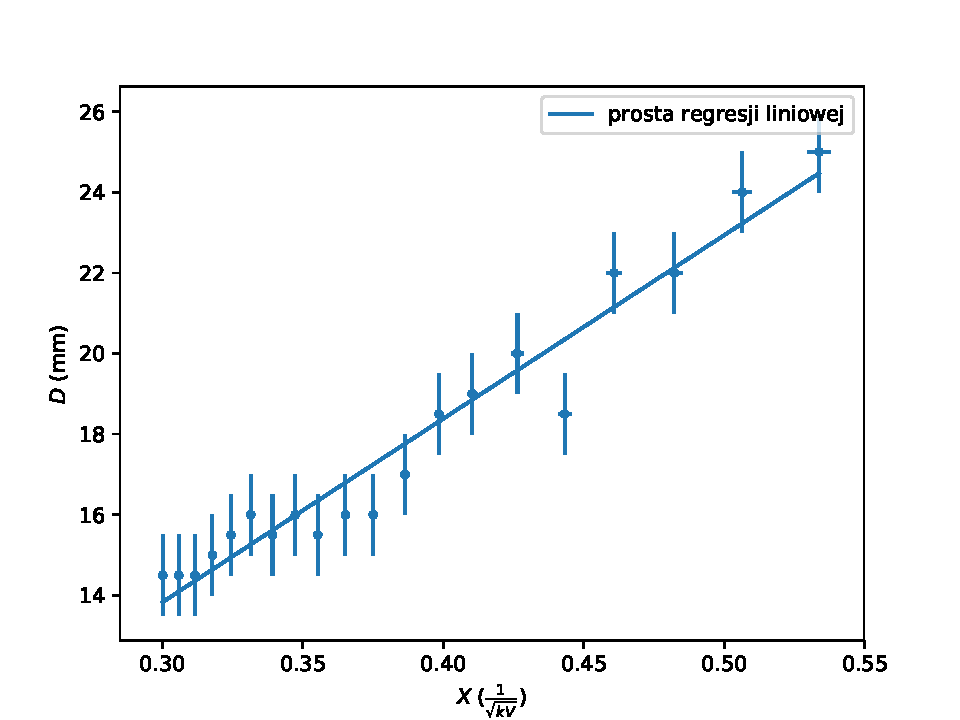
\includegraphics[scale=0.7]{wykres_A.pdf}
\caption{Wyliczona prosta regresji liniowej zestawiona wraz ze zmierzonymi wartościami dla serii $A$.}
\label{wykres_A}
\end{figure}

\begin{figure}[h]
\centering
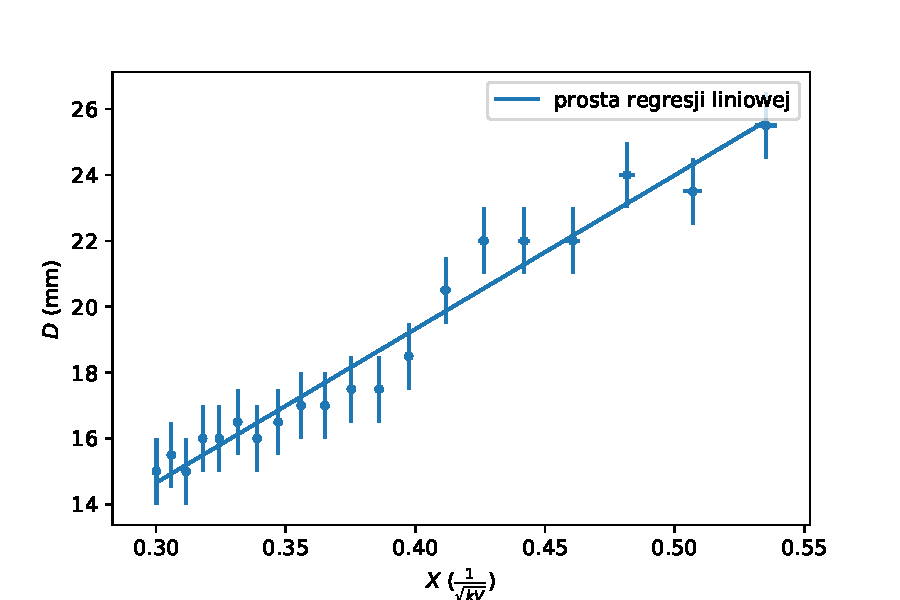
\includegraphics[scale=0.7]{wykres_B.pdf}
\caption{Wyliczona prosta regresji liniowej zestawiona wraz ze zmierzonymi wartościami dla serii $B$.}
\label{wykres_B}
\end{figure}

\subsection{Odległości między płaszczyznami atomowymi}

Ustalmy $a = 45.5$ mm$\sqrt{\text{kV}}$ oraz $u(a) = 2.5$ mm$\sqrt{\text{kV}}$.
Przekształcając wzór $a = \frac{rh}{d} \sqrt{\frac{2}{me}}$ w celu wyliczenia $d$, uzyskujemy:

$$d = \frac{rh}{a} \sqrt{\frac{2}{me}}$$

W celu wyliczenia tej wartości, posłużymy się następującymi wartościami i stałymi wraz z niepewnościami\footnote{wartości -- o ile nie zaznaczono inaczej -- pochodzą z National Institute of Standards and Technology (\url{https://physics.nist.gov/cuu/Constants/index.html}); dostęp 2018-05-04}:

\begin{itemize}
	\item odległość folia--ekran\footnote{wartość z instrukcji do laboratorium}: $r = 127$ $(3)$ mm;
	\item stała Plancka: $h = 6.626 070 040$ $(0.000 000 081)$ $10^{-34}$ Js;
	\item masa elektronu: $m = 9.109 383 56$ $(0.000 000 11)$ $10^{-31}$ kg;
	\item ładunek elementarny: $e = 1.602 176 6208$ $(0.000 000 0098)$ $10^{-19}$ C.
\end{itemize}

Ponownie skorzystamy z prawa propagacji niepewności, oznaczając przez $u(r), \dots, u(e)$ podane wyżej niepewności:

\begin{align*}
	u(d) &= \sqrt{
		\left( \frac{\partial d}{\partial r} \right)^2 \cdot u^2(r) +
		\left( \frac{\partial d}{\partial h} \right)^2 \cdot u^2(h) +
                \left( \frac{\partial d}{\partial a} \right)^2 \cdot u^2(a) +
                \left( \frac{\partial d}{\partial m} \right)^2 \cdot u^2(m) +
                \left( \frac{\partial d}{\partial e} \right)^2 \cdot u^2(e)
	} \\
	% obliczenia po drodze; zakomentowane, bo się nie mieszczą na szerokość na A4
	%&= \sqrt{
		%\left( \frac{h}{a}\sqrt{\frac{2}{me}} \right)^2 \cdot u^2(r) +
		%\left( \frac{r}{a}\sqrt{\frac{2}{me}} \right)^2 \cdot u^2(h) +
		%\left( \frac{hr\sqrt{\frac{2}{me}}}{a^2} \right)^2 \cdot u^2(a) +
		%\left( \frac{hr}{\sqrt{2e}am^{\frac{3}{2}}}  \right)^2 \cdot u^2(m) +
		%\left( \frac{hr}{\sqrt{2m} a e^{\frac{3}{2}}} \right)^2 \cdot u^2(e)
	%} \\
	&= \sqrt{
		\frac{2h^2}{mea^2} \cdot u^2(r) +
		\frac{2r^2}{mea^2} \cdot u^2(h) +
		\frac{2h^2r^2}{mea^4} \cdot u^2(a) +
		\frac{h^2r^2}{2e a^2 m^3} \cdot u^2(m) +
		\frac{h^2r^2}{2m a^2 e^3} \cdot u^2(e)
	} \\
	% jednostka: 0.04472 metra
	&\approx 1.8311440172431663 \cdot 10^{-11} \, \text{m} \\
	&\approx 0.19 \text{Å}
\end{align*}

Ostatecznie odległość między płaszczyznami atomowymi wynosi:

$$d = 3.06 \, (0.19) \, \text{Å}$$

Porównując ten wynik z dostępnymi w internecie\footnote{\url{https://hypertextbook.com/facts/2001/AliceWarrenGregory.shtml}; dostęp 2018-05-04}
($3.35$ Å)
i w publikacjach\footnote{de Boer, J. H. (1940), Atomic distances in small graphite crystals and the nature of the bond. Recl. Trav. Chim. Pays-Bas, 59: 826-830. doi:10.1002/recl.19400590903}
($3.345$ Å)
-- oraz biorąc pod uwagę, że dokładna wartość zależy od użytego grafitu --
możemy przyjąć, że wyliczona wartość jest możliwa dla grafitu użytego w laboratorium.

\section{Wnioski}

\subsection{Prawdziwość hipotezy de Broglie'a}

Rysunek \ref{wykres_A} oraz na Rysunek \ref{wykres_B} wskazują na liniową zależność między odwrotnością pierwiastka napięcia a średnicą widocznych promieni.
Dodatkowo, biorąc pod uwagę wyliczone niepewności prostej regresji liniowej, nie mamy podstaw do odrzucenia hipotezy de Broglie'a.

\end{document}
